\section{Approach} 
\label{sec:methodology}

% We envision that our efforts in prototyping an end-to-end infrastructure across the edge-to-HPC continuum can be the resulting work as paving the way for system software and adaptive resource management to become essential in creating a \textit{resilient, efficient, and integrated research infrastructure} to capture the transformative potential of the computing continuum. Based on experiments and techniques utilized for Waggle and Argo Node Resource Manager (NRM)~\cite{argo-ipdps-2019}, the following key properties and capabilities are critical for a new middleware to connect AI@Edge and HPC to user facilities: 1) limited resources in edge devices must be arbitrated by an \emph{agent running within each device}, 2) application-specific AI workloads must become \emph{reconfigurable}, and 3) OS-level services must dynamically improve edge devices, allowing each experiment to reach an optimal use of its limited resources.

We design a computing framework targeting scientific edge computing, as shown in Fig.~\ref{fig:infrastructure}, to facilitate resource monitoring and control and support the core capabilities described in Section~\ref{sec:usecase}. We leverage existing tools for the basis of our framework, including Kubernetes for container orchestration, Prometheus for resource monitoring, and a vendor runtime for inference execution. On top of that, we deploy NRM~\cite{Argo}, an infrastructure for monitoring and control of arbitrary resources. This infrastructure enables us to deploy a set of custom performance-monitoring capabilities through application instrumentation, as well as custom controls (container deployment) and a custom \textit{control policy} to adapt the system dynamically while observing how applications progress toward a science goal. The following subsections describe the resource management and control delivered through this framework.

\begin{figure}[tb]
  \centering  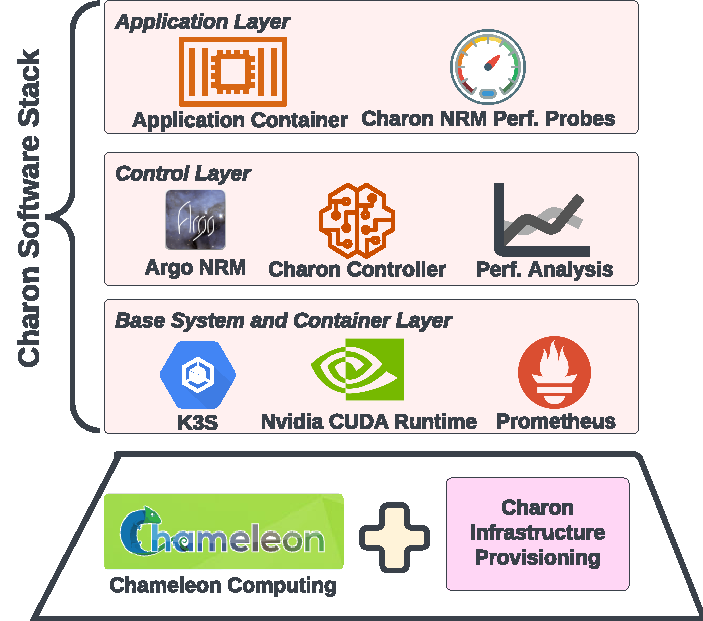
\includegraphics[width=0.9\linewidth]{figures/infrastructure.pdf}
  \caption{Charon software stack. The Charon controller is the main entity governing the resource while monitoring the performance of the system and applications.}
  \label{fig:infrastructure}
\end{figure}


\subsection{Resource Arbitration for AI@Edge}

Our system software runs as a privileged service on each node, monitoring and controlling resources. Each running agent optimizes the system performance through low-level actions in a semi-autonomous closed loop. Each agent has two main duties: 1) translating a set of resource requirements for each AI@Edge workload into a resource arbitration policy for a node and 2) providing methods to dynamically adapt this policy to reach a semi-stable resource allocation during the execution of an experiment.

% \aim{Operational Node-Level Resource Management---We will research, design, and demonstrate an agent that can dynamically allocate resources to AI@Edge workflows according to their needs as well as monitor their performance.}


\begin{figure}[tb]
  \centering
    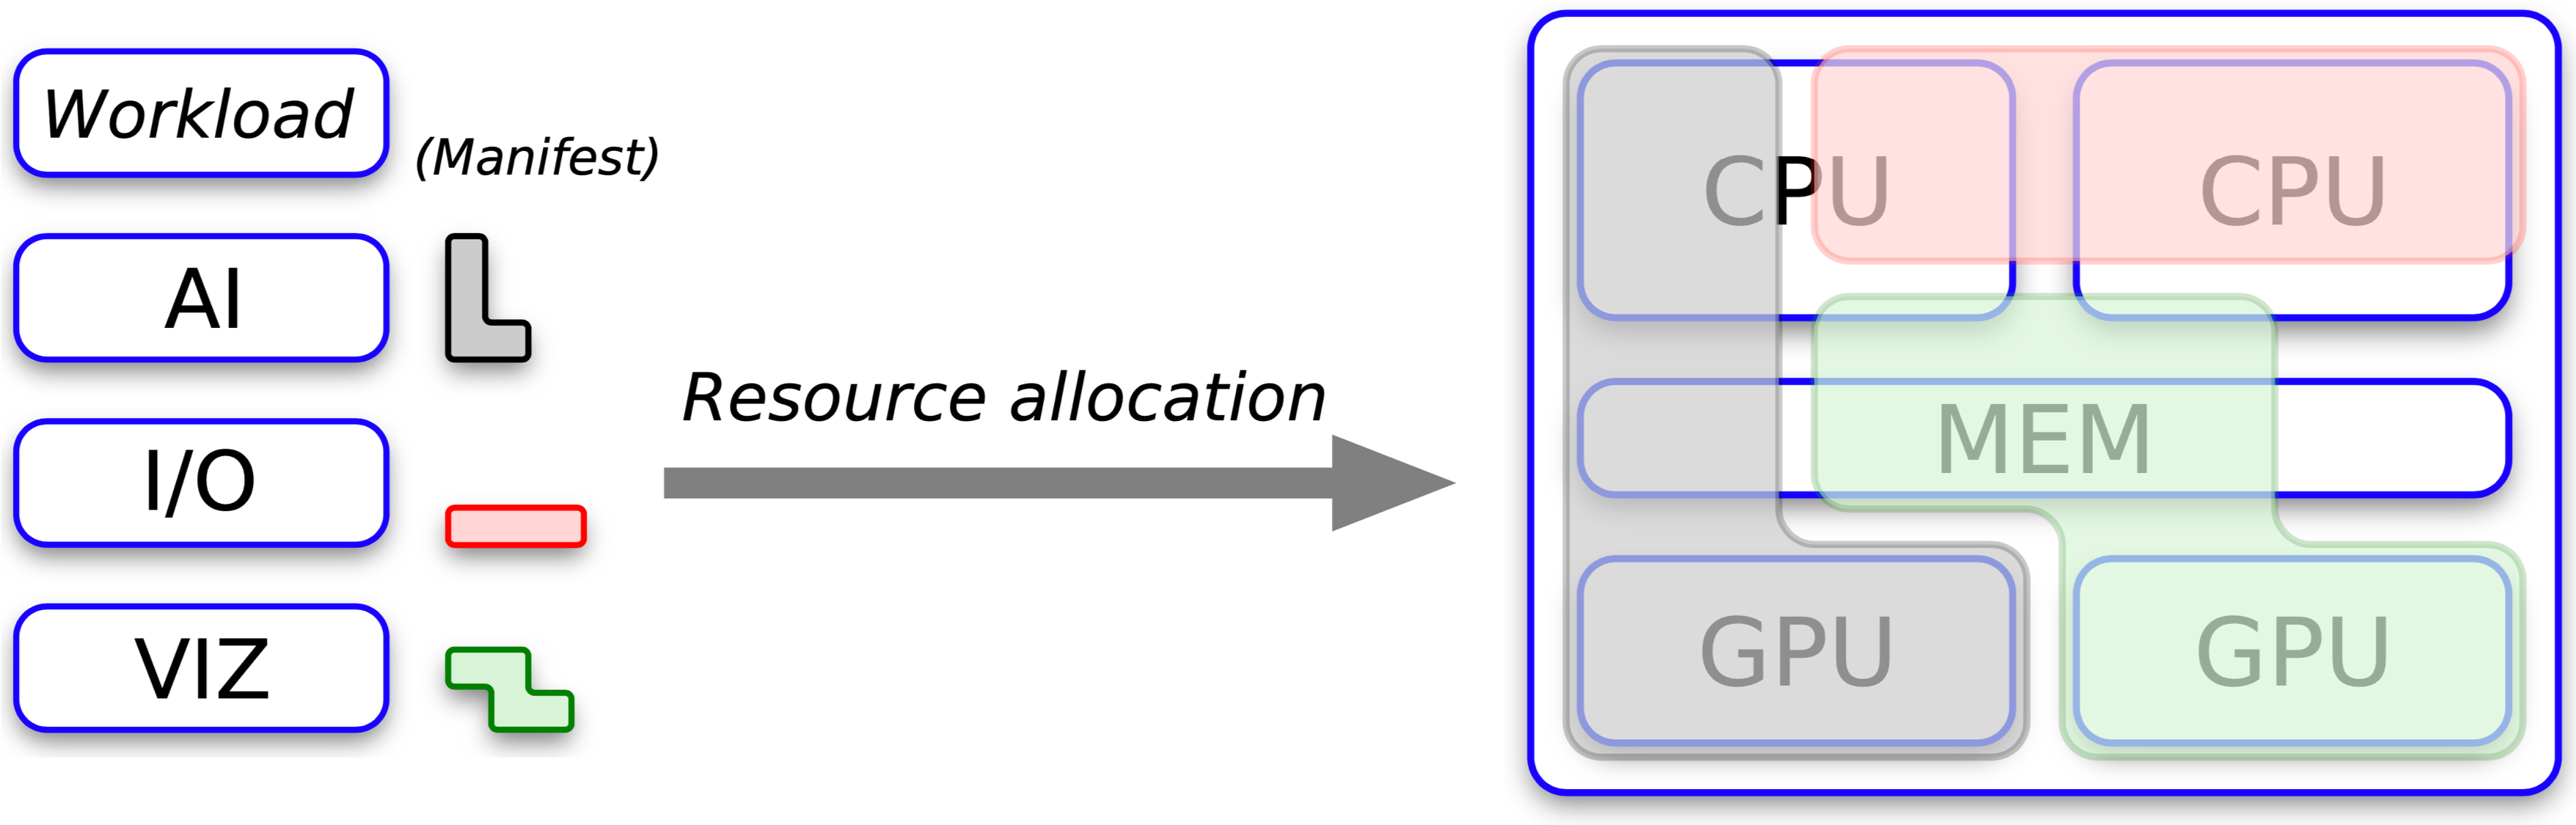
\includegraphics[width=1\linewidth]{figures/allocation-initial.png}
  \caption{System services allocate resources to an AI workload on edge devices. Each component of the workflow describes
  an initial resource request and performance metrics.}
  \label{fig:resource-allocation}
\end{figure}


\textbf{Resource Allocation and Monitoring} 
Following the design of the Waggle edge scheduler~\cite{kim2022goal}, user workloads deployed on edge nodes are expressed as a set of resources that need to be allocated, as shown in Fig.~\ref{fig:resource-allocation}. This is not a job scheduler with backfilling policies but, instead, a controller dynamically satisfying the constraints of each component of a workflow. Along with the edge scheduler, we deploy NRM, a system service that centralizes monitoring and control of node-level resources to collect information including self-reported application progress signals and power monitoring through OS-level interfaces. The NRM deployment is modular: since the infrastructure allows for arbitrary sources of information and controls, it can act as a central source of information to push into Prometheus, including application instrumentation to monitor inference performance (image per second),  data pipeline performance (data generation rate, and pipeline buffers utilization), as well as CPU and GPU occupation.

By combining the two services (Kubernetes and NRM), we deploy an infrastructure that can launch applications and rebalance their resource needs at run time, both within and across edge nodes. Since Waggle nodes run Linux and we have privileged access to the nodes, most of our control knobs are OS mechanisms for resource allocation. We directly extend the NRM to control applications the way the Waggle scheduler is launching them: as Kubernetes Pods, with the full gamut of resource arbitration mechanisms available under this interface. 


% \begin{table}[htbp]
% \caption{Typical inputs and outputs available to an edge agent.}
% \label{tab:kaa_io}
% \begin{center}
% \begin{tabular}{|c|c|}
% \hline
% \textbf{Type} & \textbf{Description} \\ \hline
% Input & Monitoring of edge environment (local sensors, power, network performance) \\ \hline
% Input & Monitoring of group of nodes under control (data services, health of the system) \\ \hline
% Input & Monitoring of application components under control (AI performance)\\ \hline
% Input & User-provided policies and performance constraints\\ \hline
% Output & Actions on knobs under our control (local and remote) \\ \hline
% Output & Actions on application tunables under our control (if available) \\ \hline
% Feedback & Monitoring information sent to edge management infrastructure \\ \hline
% \end{tabular}
% \end{center}
% \end{table}

% \vspace{5pt}
% \aim{Dynamic Node-Level Adaptation---We will research, design, and demonstrate methods for edge agents to search for better resource allocations dynamically, while preserving performance requirements.}

%\paragraph{\textbf{Adaptive Optimization}}
\textbf{Adaptive Optimization} Our edge agent optimizes the use of computing resources at run time for performance and stability. Given a set of performance metrics for application components, the agent monitors performance and takes actions to improve computing performance following policies set by users as shown in Fig.~\ref{fig:resource-optimization}, mostly by rebalancing of resources or the activation/deactivation of certain hardware features. Similarly, prioritizing a specific workload or fair distribution of computing resources across users, throughput, or reliability optimizes computing performance in a multitenant configuration.

Many design choices impact the performance, stability, and flexibility of resource management policies. First, the nature of the inputs has an impact: some metrics are discrete or have fixed domains (min, max, or both), while some others are noisy in value or time (arrival time), available at fixed rates (sampling) or event-based (tracing). A choice can also be made regarding computing statistics across time windows or deriving metrics from multiple signals, while a specific signal can trigger a new decision, or decisions can be made at regular time intervals. Control knobs in our service exhibit similar characteristics.

Second, the policy itself can take various forms, depending on the number of inputs (signals) and outputs (controls) supported, from instantaneous models that directly map signals to control values regardless of the time dimension, to control theory designs such as PID controllers that can smooth out the control over longer periods~\cite{europar21, ccta22}, or reinforcement learning policies~\cite{ic2e23} that can take into account the cost of the entire sequence of actions in their process.

Third, some control loop designs can be more amenable to swapping inputs or outputs, while others embed assumptions about the nature of the system that need to be revisited when applied elsewhere. Some policy designs can offer strong guarantees of the stability of the control when the environment changes, while others require preventing inputs or controls from going out of bounds.

We do not aim for a single policy design that could adapt to any experiment or scientific workflow objective. Instead, our infrastructure is designed to allow users to specify which system observations and controls should be relevant to their use case and the policy itself.

% Leveraging our experience in building both policies based on control theory~\cite{europar21, ccta22} and using online reinforcement learning~\cite{ic2e23} we will research and demonstrate policies that strive to be adaptable to a wide range of use cases. We will also take advantage of the flexibility of the Argo NRM infrastructure, which separates the handling of metrics (monitoring), actions (control knobs) and the policies themselves, allowing us to quickly experiment with one aspect of the control design without impacting the others.


\begin{figure}[!t]
  \centering
  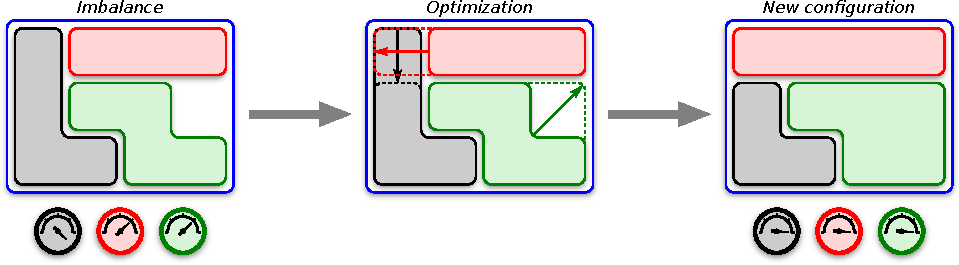
\includegraphics[width=1\linewidth]{figures/allocation-optimize.pdf}
  \caption{Based on the observed performance of the system and available controls (left), our system services periodically optimize the resource allocation (center), resulting in an improved configuration (right).}
  \label{fig:resource-optimization}
\end{figure}


\subsection{AI@Edge Reconfiguration}

Our use case includes AI models deployed at the edge and involves steering instruments. It also includes workflows where the model steering the experiment can be updated at run time based on additional tuning and training done on HPC systems. In these cases, during the lifetime of an experiment, a workflow system will be in charge of sending collected data to HPC resources, retraining the models, and shipping the updated models back to the edge~\cite{babu2022deep}. We envision this pipeline as a set of system services running on edge nodes and in an HPC compute environment and bridging the two environments together. Two main challenges that need to be addressed for such a design to succeed are 1) creating a data and model management infrastructure that can maintain information provided by users about the curation of data and models and 2) developing methods to update and adapt the configuration of edge devices when such a workflow triggers actions as shown in Fig.~\ref{fig:ai-updates}.

\begin{figure}[tb]
  \centering
    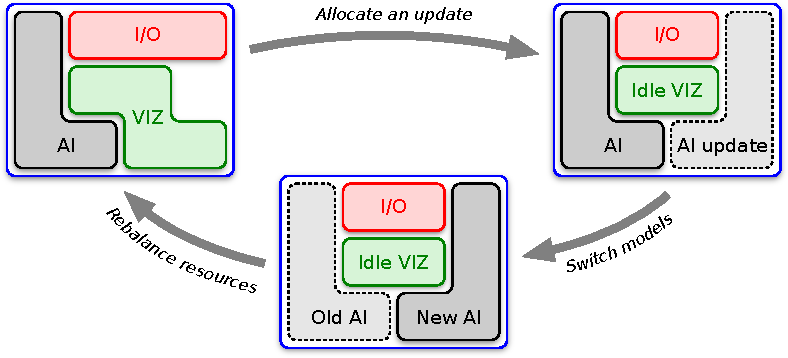
\includegraphics[width=1\linewidth]{figures/ai-reconfiguration.pdf}
    \caption{Updating the AI@Edge model while ensuring continuous operation and performance: resources need to be reprioritized during and after the update received from an HPC system.}
   \label{fig:ai-updates}
\end{figure}

% \aim{Data and Model Management---We will explore the most flexible methods allowing users to connect edge devices and HPC systems, moving data, models, and tuning workflows across the computing continuum.}

\textbf{An Infrastructure for Model Management}
Which data to move, how to retrain a model, and when to retrain or replace a model are decisions best made by experts in their respective domain sciences and their particular experiments. This information, however, can be provided to an infrastructure that can then act on such policies while ensuring the performance and reliability of the surrounding environment. A function as a service (FaaS) component in the infrastructure can monitor the state and data produced by an experiment and be dynamically triggered to move the data to an HPC system and launch the tuning of AI components and their update. This infrastructure will have to take into account timing and performance constraints such as the volume of data that needs to be moved (inputs and model), the time needed to move it, and the required resources. Indeed, we expect that, depending on the models being updated and the nature of both the HPC resources and the edge nodes, such infrastructure might operate at differing timeframes.

% Note that we expect data streaming infrastructures to be already present in most cases, after all ASCR has funded projects to design them, including the High Performance Data Facility. We aim here for the \textit{integration} of these services into our infrastructure, from designing the mechanisms to dynamically adjust resources for model updates and data services, to developping a better understanding of their resource requirements and how we can cooperate so that AI@Edge workloads continue to perform as required when additional services are sharing resources.

% \aim{Stretch Goal---We will explore how various models and edge device configurations impact resource utilization, the need for resource arbitration, and the stability of resource requirements across an experiment lifetime.}

\textbf{Sources of Variability at Run Time and Edge Capabilities}
The capabilities of edge devices (their hardware configuration) and similarly the capabilities of AI models (architecture, size) are always changing: new AI methods are developed, new accelerators become available, and instruments are updated (e.g., the ongoing APS upgrade). We expect that these changes will have an impact on the constraints and performance of our solution in the future. The flexibility of our infrastructure will be an asset in such cases, as new sources
of monitoring data or controls can be added easily.

% As a stretch goal, we will characterize how these types of changes, either in hardware or methods, impact our design; we will use this as an opportunity to generate priority research directions for this type of work under future funding.
% We recognize that we may not be able to extract sufficient information from existing literature alone. Therefore, we plan to run the candidate AI models for the staging nodes on available AI accelerators at Argonne. Fortunately, the Argonne AI Testbed provides state-of-the-art infrastructure of next-generation AI accelerators, including cutting-edge systems such as Groq, SambaNova, GraphCore, Habana Gaudi, and Cerebras (see Appendix~\ref{sec:facilities}). 

We acknowledge that some experiments might require real-time response
behavior or might involve considering more than just average performance or
short-term measurements for proper resource management. We intend to develop the
infrastructure further toward those goals.

% For example, Figure~\ref{fig:braggnnongroq} shows end-to-end latency measurements for the BraggNN model running on the Groq TSP accelerator; while the latency is fairly uniform during most of the 1,000 inferences, we can observe several spikes, which could negatively impact scientific experiments, particularly those involving real-time lab automation. Therefore, we will assign students to perform similar measurements on other AI accelerators to comprehensively assess systemwide characteristics.

% \begin{figure}[tb]
%     \includegraphics[width=0.45\textwidth]{figures/bnn-ts-Groq-base.png}
%     \includegraphics[width=0.45\textwidth]{figures/bnn-ts-Groq-nb.png}
%     \caption{Measuring the inference latency of the BraggNN model running on the Groq TSP accelerator: baseline implementation (left) and optimized one (right).}
%     \label{fig:braggnnongroq} 
% \end{figure}
